\chapter{Proposta de Solução}

O presente capítulo detalha a modelagem da solução e a arquitetura proposta. A primeira Seção~\ref{section:modelagem} apresenta os diagramas que foram construídos a partir das duas fases da metodologia MASE. A segunda Seção~\ref{section:arquitetura} mostra a arquitetura da solução em um escopo mais geral, considerando além do SMA a plataforma~\emph{web} e a sua comunicação.

A arquitetura básica do sistema já havia sido previamente decidida de acordo com~\cite{editalFrank}, bem como o nome da solução:~\emph{Frank}. Basicamente, a aplicação funciona da seguinte forma: O aluno deverá autenticar-se em uma plataforma~\emph{web} para a determinação do seu estilo de aprendizagem. Em seguida, o professor autentica-se na plataforma e verifica o estilo de aprendizagem dos seus alunos. A verificação do estilo de aprendizagem e manutenção do modelo multidimensional é feita por agentes. Logo, a solução proposta foi desenvolvida em duas aplicações:~\emph{Web} e SMA.

A aplicação SMA é baseada em grupos de trabalho por aluno. Após a autenticação do aluno na plataforma~\emph{web}, o SMA realiza a criação dos agentes do grupo de trabalho designado para ele. Esses agentes são responsáveis pela manutenção do modelo multidimensional do aluno na plataforma e são atualizados conforme ocorre o envio de dados dos ambientes externos para os agentes do grupo de trabalho.

Após a escolha da metodologia MASE, justificada no capítulo 2, foram elicitados todos os requisitos e regras a partir de~\cite{editalFrank}, onde foi compreendido inicialmente o problema. Em seguida, uma série de artefatos foram gerados em consonância com a metodologia até o último passo, a geração dos agentes. Ao fim da metodologia, a solução foi composta por sete diferentes tipos de agentes:
\begin{enumerate}
	\item \emph{GatewayAgent} - Agente responsável pela interface com a plataforma web que irá interagir com os alunos e docentes.
	\item \emph{WebServiceAgent} - Agente responsável pela interface com o Ambiente Virtual de Aprendizagem.
	\item \emph{ManagerAgent} - Agente responsável pelo controle da plataforma
	\item \emph{WorkgroupAgent} - Responsável pelos agentes cognitivo, afetivo e metacognitivo.
	\item \emph{CognitiveAgent} - Responsável pelo modelo cognitivo do aluno.
	\item \emph{MetacognitiveAgent} - Responsável pelo modelo metacognitivo.
	\item \emph{AfectiveAgent} - Responsável pelo modelo afetivo.
\end{enumerate}

O primeiro agente,~\emph{GatewayAgent}, é responsável pela interação direta com a plataforma web. Essa plataforma irá interagir com os alunos (por meio de questionários de estilo de aprendizagem) e docentes (notificando o estilo de aprendizagem dos seus alunos) e encaminhará os dados para o agente em questão, que repassará ao ambiente.

O agente interface~\emph{WebServiceAgent}, é responsável pela comunicação com os web services do SMA Frank, que é a forma escolhida para futuras interações com AVA. Por fim, o agente~\emph{ManagerAgent} é responsável pela criação dos agentes.

A partir dos agentes e regras gerados, foi implementado o SMA na linguagem JAVA utilizando o~\emph{framework} JADE. Em seguida, foi desenvolvido a plataforma~\emph{web} utilizando~\emph{JBoss Seam}, responsável pela interface do grupo de trabalho de agentes com o aluno. Após a conclusão da plataforma, foi necessário integrar as duas aplicações por meio do módulo~\emph{JadeGateway} disponibilizada nativamente pelo JADE.

Por fim, a solução foi testada por meio de cenários que simulavam o uso por meio dos atores Aluno e Docente. A demonstração foi feita a partir do mapeamento do estilo de aprendizagem de um aluno e em seguida do docente visualizando o estilo de aprendizagem dos alunos de sua turma.

As seções seguintes detalham a metodologia, justificam a arquitetura da solução por meio da modelagem definida na metodologia MASE.

\section{A Modelagem}\label{section:modelagem}

A modelagem foi desenvolvida utilizando-se a ferramenta~\emph{agentTool}. A ferramenta possui meios para diagramar todas as fases e passos do MASE, auxiliando o analista em todos os diagramas necessários, além de gerar código automático para alguns frameworks de SMA.

A metodologia é dividida em duas fases: Análise e Projeto. Na primeira Seção~\ref{subsection:analise} é desenvolvida a fase de análise responsável pelo levantamento de requisitos e entendimento das regras e tarefas. A segunda fase, na Seção~\ref{subsection:design}, é responsável pela criação dos agentes, conversações e componentes internos.

\subsection{Análise}\label{subsection:analise}

A metodologia inicia-se com o passo de captura das metas. Para tanto, foi necessário primeiramente um levantamento inicial dos requisitos do SMA. Os requisitos foram levantados e compreendidos por meio da sua documentação inicial~\cite{editalFrank}, onde é possível listar:

\begin{enumerate}
	\item O sistema deve manter um modelo do estudante, onde será determinado o seu estilo de aprendizagem e será notíficado ao docente.
	\item O sistema deve assistir (auxiliar) o aluno por meio de um grupo de trabalho.
	\item O sistema deve fazer interface com Ambiente Virtual de Aprendizagem, a fim de estabelecer comportamentos do estudante.
	\item O sistema deve criar uma modelagem cognitiva do aluno, onde são mantidas informações sobre o desempenho, de acordo sua interação em Ambiente Virtual de Aprendizagem, e informações a respeito do seu estilo de aprendizagem.
	\item O sistema deve criar uma modelagem metacognitiva do aluno, onde são armazenadas informações com o intuito de melhorar processos de aprendizagem de domínios específicos.
	\item O sistema deve criar uma modelagem afetiva do estudante, especificamente a respeito da modelagem da personalidade e emoções do estudante.
	\item O sistema deve fazer interface com Ambiente Virtual de Aprendizagem.
	\item O sistema deve refutar ou confirmar o estilo de aprendizagem do aluno a partir do desempenho relacionado à interação com o sistema e/ou com Ambiente Virtual de Aprendizagem.
	\item O sistema SMA deve atualizar o modelo do estudante com base em mapeamentos a partir dos registros de trabalho do estudante.
	\item O sistema deve construir o modelo do estudante a partir de uma modelagem explícita, ou seja, a partir do feedback explícito do estudante (questionário).
	\item O sistema deve construir o modelo do estudante a partir de uma modelagem implícita, ou seja, a partir do desempenho obtido nas ferramentas de aprendizado.
\end{enumerate}

A partir destes requisitos, foi possível estabelecer metas que o sistema deveria atingir para satisfazê-los:

\begin{enumerate}
	\item Manter um modelo do estudante.
	\item Auxiliar o aluno por meio de um grupo de trabalho (Workgroup).
	\item Notificar ao docente.
	\item Interface com ambientes de virtuais de aprendizagem.
	\item Interface com o Aluno.
	\item Criar modelagem cognitiva.
	\item Criar modelagem metacognitiva.
	\item Criar modelagem modelagem afetiva.
	\item Criar modelagem da personalidade.
	\item Criar modelagem das emoções do estudante.
	\item Confirmar estilo de aprendizagem do aluno.
	\item Refutar estilo de aprendizagem do aluno.
	\item Construir modelo de desempenho do aluno.
	\item Construir modelagem explícita.
	\item Construir modelagem implícita.
	\item Construir modelo de estilo de aprendizagem do aluno.
\end{enumerate}

A partir do levantamento, foi possível observar que a meta 1 abrange o escopo geral de toda a aplicação, sendo possível estabelecer como meta do sistema. A meta 2 indica que o SMA deverá criar um grupo de trabalho para cada aluno que estiver usando o sistema. O grupo de trabalho deve ser composto pelos agentes cognitivo, afetivo e metacognitivo, onde cada um possui suas respectivas metas. No levantamento, foram previstas três interfaces: Interface~\emph{web} com o Aluno, notificação do docente (via~\emph{web}) e interface com ambientes de virtuais de aprendizagem.

A hierarquia de metas do SMA Frank, apresentada na Figura~\ref{fig:metas-frank}, foi desenvolvida para graduar as metas que podem ser atingidas com o cumprimento de outras. Os retângulos em cinza representam metas particionadas.

\begin{sidewaystable}
	\centering
	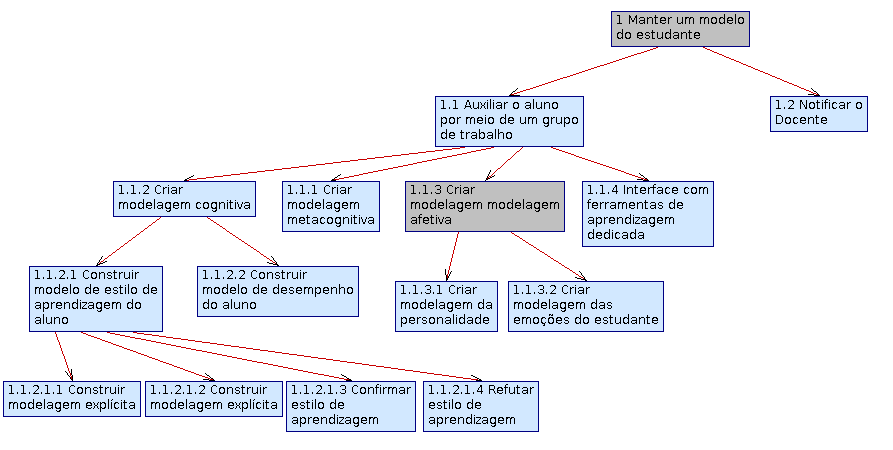
\includegraphics[scale=0.7]{images/metas-frank.png}
	\caption{Hierarquia de Metas do SMA Frank.}
	\label{fig:metas-frank}
\end{sidewaystable}

Foram levantados 5 principais casos de uso, alguns com fluxos alternativos que representam fluxos alternativos no caso de uso, mas não necessariamente implicam em uma execução no SMA, apenas na parte~\emph{web}, como por exemplo: Erro de Login. Para fins de detalhamento, este trabalho utiliza-se da notação completa de desenvolvimento de casos de uso.

O primeiro caso de uso, descrito na Apêndice~\ref{chapter:uc1}, diz respeito à modelagem cognitiva do aluno. Existem dois cenários possíveis: Modelagem implícita (principal cenário de sucesso) e modelagem explícita (cenário alternativo). O SMA deverá processar o questionário de estilos de aprendizagem, respondido pelo aluno, para mapear explicitamente o seu modelo cognitivo a partir das suas respostas e então obter o seu modelo cognitivo.

O segundo caso de uso, descrito no Apêndice~\ref{chapter:uc2}, descreve o cenário de notificação do docente. Nele, o docente é autenticado no sistema e o sistema exibe uma lista de alunos disponíveis nas mais diversas turmas. O docente seleciona um aluno e então o sistema exibe os dados relativos ao modelo do aluno.

O terceiro caso de uso, descrito respectivamente no Apêndice~\ref{chapter:uc3}, dizem respeito à inferência do modelo afetivo. De forma análoga, o caso de suo descrito em~\ref{chapter:uc4} ilustra a inferência do modelo metacognitivo do aluno.

O Apêndice~\ref{chapter:uc5} descreve o último caso de uso que foi levantado para promover a interação entre os diferentes AVA e o SMA Frank. Devido a possibilidade dos AVA serem desenvolvidos em qualquer linguagem, é necessário utilizar-se de uma forma de comunicação comum entre aplicações.

Logo o SMA Frank irá utilizar de~\emph{WebServices} para a comunicação externa, garantindo que diversas aplicações poderão interagir com o SMA. Para novos AVAs, tudo o que precisará ser feito é a implementação da assinatura do serviço no~\emph{WebService}. Dessa forma a solução garante uma intervenção mínima no código do AVA, exigindo menos tempo na codificação da comunicação e garantindo o foco na inferência à ser feita pelo SMA.

Após o desenvolvimento dos casos de uso, foi necessário refinar os diagramas de sequência. Todos os diagramas foram desenvolvidos na ferramenta~\emph{agentTool}, visto que ele acompanha todas as fases do MASE. Para o primeiro caso de uso, foram desenvolvidos dois diagramas de sequência distintos: Um para o fluxo principal e outro para o fluxo alternativo.

No diagrama de sequência do caso de uso 1, apresentado na Figura~\ref{fig:dss-uc1-fluxo-principal}, existem 6 regras. O fluxo do Sistema inicia-se com a regra~\emph{StudentInterface}, onde ele envia os dados de questionário para o~\emph{Manager}. Este então gera um evento de localização do aluno. Em seguida, gera o evento enviar para a regra~\emph{StudentWorkGroup}, com o parâmetro~\emph{questionário}. A regra~\emph{StudentWorkGroup} gera o evento de enviar para as regras~\emph{CognitiveAction},~\emph{AffectiveAction} e~\emph{MetacognitiveAction}. Eles retornam respectivamente os modelos~\emph{Cognitivo},~\emph{Afetivo} e~\emph{Metacognitivo}. A regra~\emph{cognitiveAction} ainda gera mais um evento de envio para a regra~\emph{LearningMethodAnalyzer}, que retorna o estilo de aprendizagem.

\begin{figure}
	\centering
	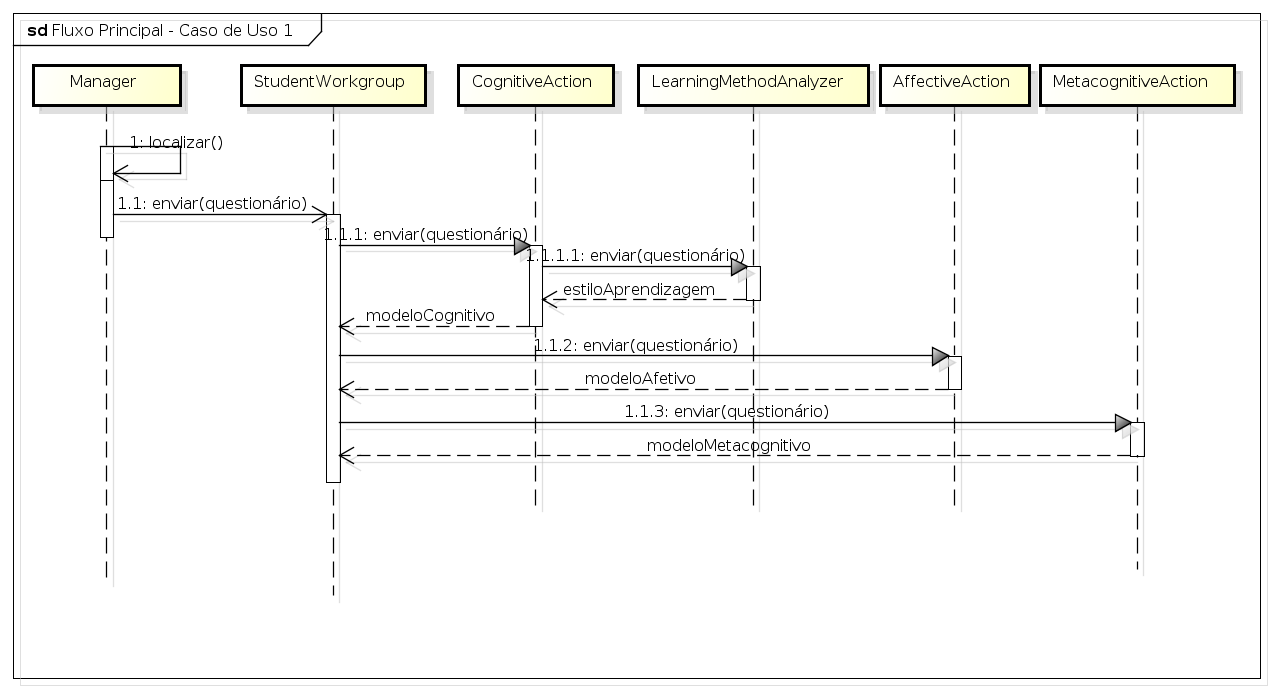
\includegraphics[scale=0.52]{images/dss-uc1-fluxo-principal.png}
	\caption{Diagrama de sequência do fluxo principal, caso de uso 1.}
	\label{fig:dss-uc1-fluxo-principal}
\end{figure}

A Figura~\ref{fig:dss-uc1-fluxo-alternativo} apresentação o fluxo de exceção do primeiro caso de uso, onde ilustra a regra~\emph{WebServiceInterface} que recebe os dados do AVA e envia para a regra Manager por meio do evento~\emph{enviar}. Após esse evento, a regra~\emph{StudentWorkgroup} recebe o evento e reenvia para~\emph{CognitiveAction}. Em seguida ele envia para as regras~\emph{LearningMethodAnalyzer} e~\emph{PerformanceAnalyzer} que vão mapear o estilo de aprendizagem e a performance. Por fim, com estes dados, o modelo cognitivo é retornado para a regra~\emph{StudentWorkgroup}.

\begin{figure}
	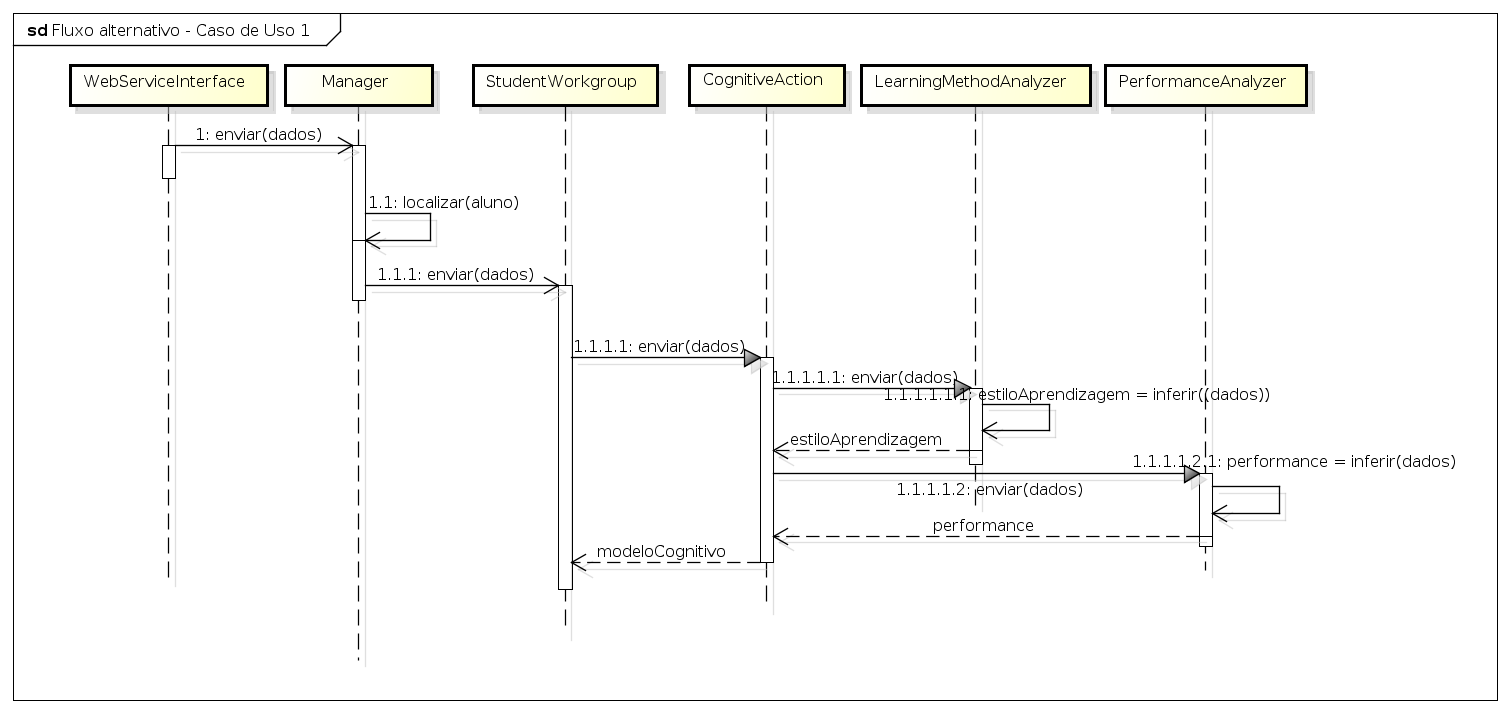
\includegraphics[scale=0.52]{images/dss-uc1-fluxo-alternativo.png}
	\caption{Diagrama de sequência do fluxo alternativo, caso de uso 1.}
	\label{fig:dss-uc1-fluxo-alternativo}
\end{figure}

A Figura~\ref{fig:dss-uc3-fluxo-principal} ilustra a inferência afetiva descrita no fluxo principal do caso de uso 3. O processo de comunicação das regras~\emph{WebServiceInterface} e~\emph{StudentWorkgroup} funciona de forma semelhante ao diagrama anterior. A regra~\emph{AffectiveAction} gera um evento de inferência de modelagem afetiva.

\begin{figure}
	\centering
	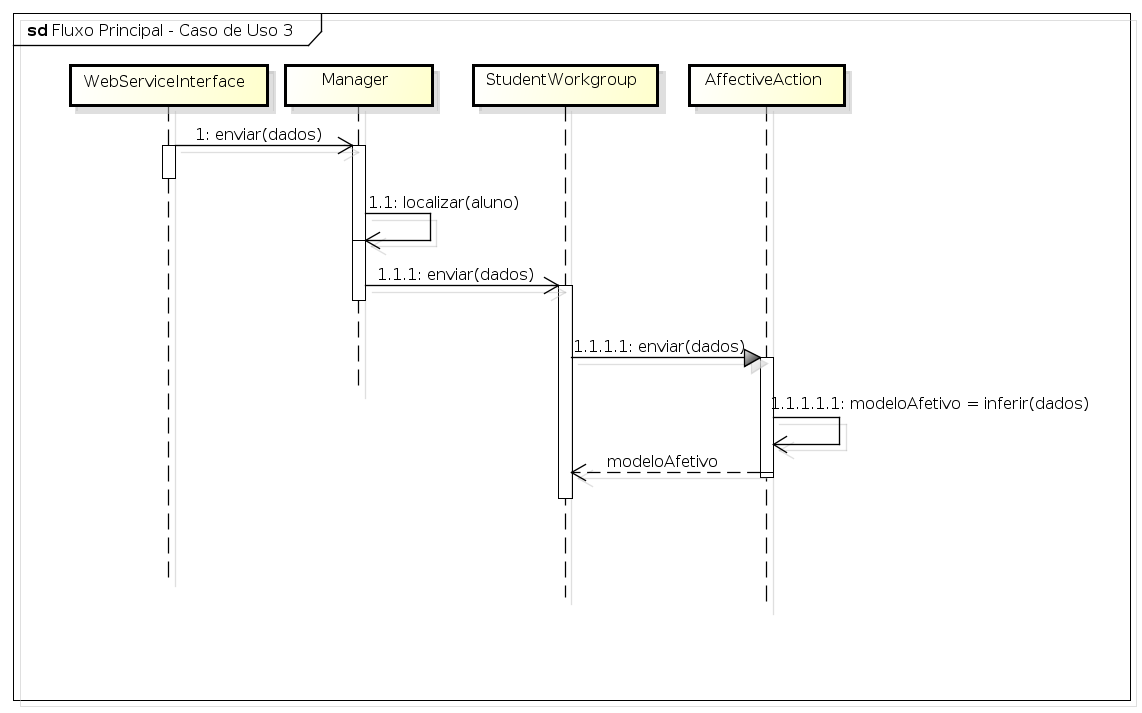
\includegraphics[scale=0.52]{images/dss-uc3-fluxo-principal.png}
	\caption{Diagrama de sequência do fluxo principal, caso de uso 3.}
	\label{fig:dss-uc3-fluxo-principal}
\end{figure}

O diagrama de sequência do fluxo principal caso de uso 4, apresentado na Figura~\ref{fig:dss-uc4-fluxo-principal}, funciona de forma similar ao caso de uso anterior, com a diferença de que a regra~\emph{MetacognitiveAction} realiza a inferência da modelagem metacognitiva.

\begin{figure}
	\centering
	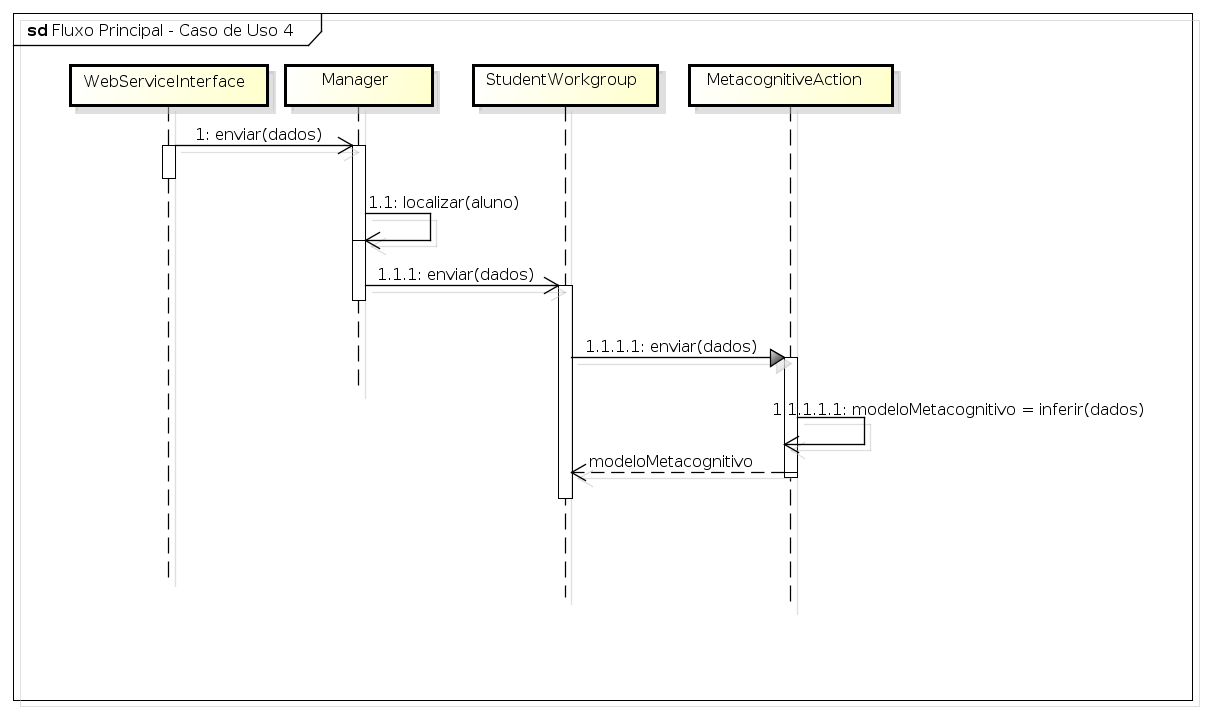
\includegraphics[scale=0.52]{images/dss-uc4-fluxo-principal.png}
	\caption{Diagrama de sequência do fluxo principal, caso de uso 4.}
	\label{fig:dss-uc4-fluxo-principal}
\end{figure}

Por fim a Figura~\ref{fig:dss-uc5-fluxo-principal} apresenta o diagrama de sequência do fluxo principal do caso de uso5. Nele é mostrado a  comunicação da regra~\emph{WebServiceInterface} com a regra~\emph{Manager}. A primeira realiza a validação de dados e em seguida o envio de dados. Após receber os dados, a regra~\emph{Manager} localiza o aluno e continua o fluxo de execução.

\begin{figure}
	\centering
	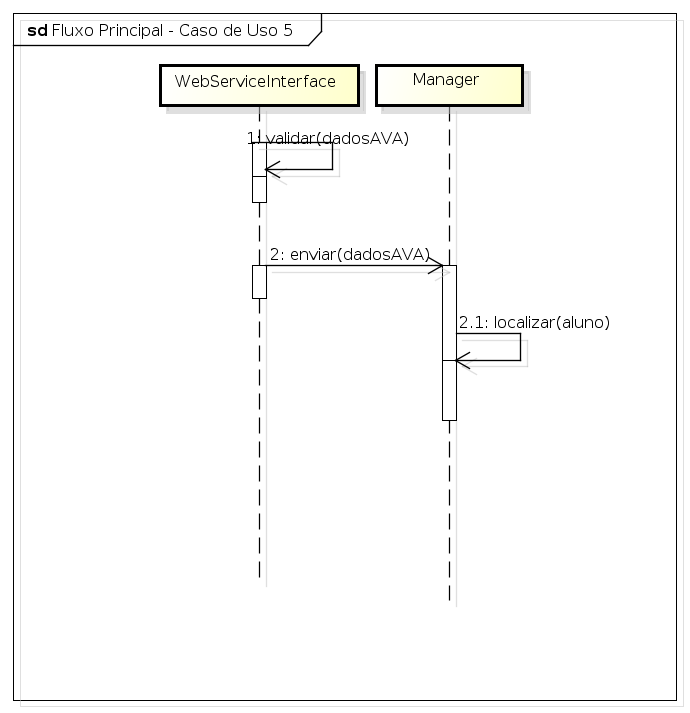
\includegraphics[scale=0.52]{images/dss-uc5-fluxo-principal.png}
	\caption{Diagrama de sequência do fluxo principal, caso de uso 5.}
	\label{fig:dss-uc5-fluxo-principal}
\end{figure}

Por fim, após o levantamento de todas as regras foi necessário criar tarefas que satisfaçam o cumprimento das regras. Em outras palavras, é necessária a criação do~\emph{MASE Role Model}. A organização das metas e tarefas foi descrita na Tabela~\ref{tabela:mase-role-model}, a qual cada linha representa as regras obtidas do diagrama, seguidas das respectivas tarefas. É importante ressaltar que, devido aos objetivos deste trabalho, houve um refinamento muito maior do agente cognitivo. Os agentes afetivos e metacognitivos foram apenas projetados na arquitetura.

\begin{table}
	\caption{Estruturação das Tarefas por Regra}
	\begin{tabular}{|p{5cm} | p{9cm}|}
		\hline
		\textbf{Regra}		& \textbf{Tarefas} \\
		\hline
		StudentInterface 	& Validar Dados, Autenticar Aluno  \\
		\hline
		WebServiceInterface 	& Validar Dados  \\
		\hline
		Manager 		& Determinar Workgroup do Aluno, Criar Workgroup do Aluno  \\ %Colocar a possibilidade de balancear o ambiente aqui
		\hline
		StudenWorkgroup 	& Processar Dados, Atualizar Modelo   \\
		\hline
		CognitiveAction 	& Separar Dados de Aprendizagem, Atualizar Modelo Cognitivo, Atualizar Performance  \\
		\hline
		MetacognitiveAction 	& Inferir Modelo Cognitivo  \\
		\hline
		AffectiveAction 	& Inferir Modelo Afetivo  \\
		\hline
		LearningMethodAnalyzer 	& Analisar Estilo de Aprendizagem  \\
		\hline
	\end{tabular}
	\label{tabela:mase-role-model}
\end{table}

A Figura~\ref{fig:frank-role-model} apresenta o~\emph{MASE Role Model}, onde é possível visualizar toda a sua estruturação das regras e tarefas. De forma geral, a regra~\emph{Manager} é a responsável pela gerência de todo o SMA. Ela pode receber os dados da regra~\emph{StudentInterface} (interface~\emph{web} da aplicação) ou~\emph{WebServiceInterface} (Interface com AVA). Além disso, a regra~\emph{StudentInterface} possui uma tarefa para autenticação do aluno, a qual encaminha uma mensagem para a regra~\emph{Manager} que cria o workgroup do aluno. As linhas tracejadas representam comunicações internas enquanto as linhas sólidas representam comunicações externas.

A regra~\emph{StudentWorkgroup} será a regra responsável pela gerência do grupo de trabalho do aluno. Ela recebe os dados da regra~\emph{Manager} e reencaminha para as regras~\emph{Cognitive},~\emph{Affective} e~\emph{Metacognitive}. As linhas tracejadas de cor azul representam comunicações internas entre as regras.

\begin{figure}
	\centering
	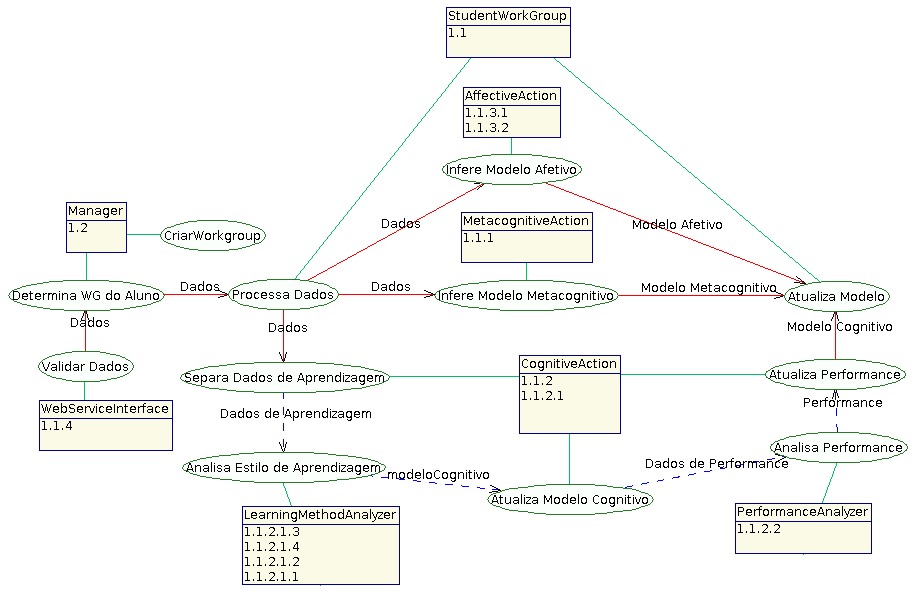
\includegraphics[scale=0.48]{images/mase-role-model.png}
	\caption{Diagrama~\emph{MASE Role Model} gerado para o SMA Frank.}
	\label{fig:frank-role-model}
\end{figure}

A ferramenta~\emph{agentTool} automaticamente indicou a criação dos~\emph{Concurrent Tasks Diagrams} para cada tarefa. O fluxo de execução pode iniciar-se nas regras~\emph{StudentInterface} ou~\emph{WebServiceInterface}. Elas representam respectivamente as interações com o Aluno e com o Ambiente Virtual de Aprendizagem.

A regra~\emph{WebServiceInterface} possui o diagrama da tarefa ``Validar Dados'', apresentado na Figura~\ref{fig:validar-dados}, inicia com o recebimento de uma mensagem de um agente ``a'' e os dados ``DadosWebService''. A tarefa passa ao estado ``ValidarDados'', onde ele recupera as variáveis ``idUsuario'' e ``status'' (verificação se o usuário é válido no ambiente). Em seguida a variável ``status'' é testada: Caso seja inválida o agente ``a'' recebe um código de erro. Caso contrário, a tarefa muda para o estado ``enviarDados'', onde ele procura o agente responśavel pela tarefa ``manager'' e encaminha os dados ``DadosWebService''
 
\begin{figure}
	\centering
	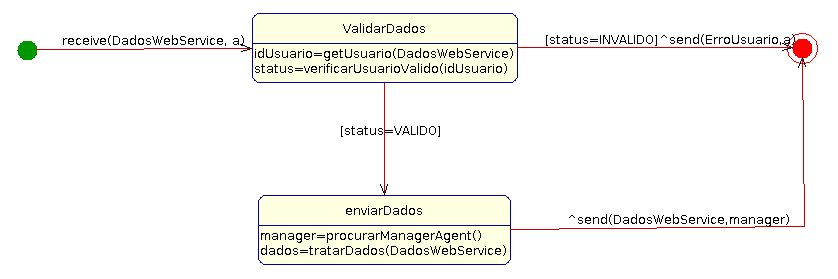
\includegraphics[scale=0.48]{images/td-validar-dados.png}
	\caption{Detalhamento da tarefa ``Validar Dados'' que pertence à regra~\emph{WebServiceInterface}.}
	\label{fig:validar-dados}
\end{figure}

A Figura~\ref{fig:td-enviar-quest} apresenta o diagrama da tarefa ``Enviar Questionário'', da regra~\emph{StudentInterface}. Ele inicia a partir de uma mensagem da plataforma~\emph{web} contendo os dados do questionário. Esses dados são convertidos para uma linguagem de ontologia do SMA. Em seguida, esse questionário é enviado para o manager.

\begin{figure}
	\centering
	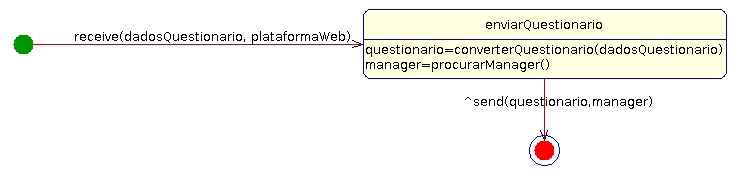
\includegraphics[scale=0.48]{images/td-enviar-quest.png}
	\caption{Detalhamento da tarefa ``Enviar Questionário'' que pertence à regra~\emph{StudentInterface}.}
	\label{fig:td-enviar-quest}
\end{figure}

Ainda na regra~\emph{StudentInterface}, a Figura~\ref{fig:td-autenticar-aluno} apresenta o diagrama da tarefa ``Autenticar Aluno'', o qual inicia com uma mensagem da plataforma~\emph{web} contendo o aluno a ser criado. A tarefa verifica a existência do aluno e em caso negativo, envia a mensagem de criação à tarefa~\emph{Manager}. Caso contrário, envia uma mensagem de erro à plataforma~\emph{web}.

\begin{figure}
	\centering
	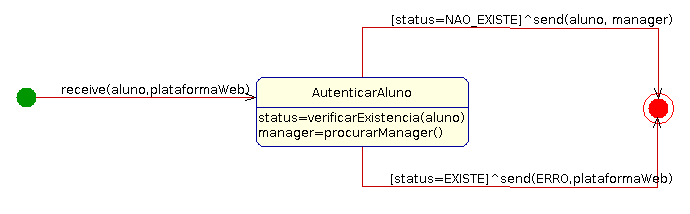
\includegraphics[scale=0.48]{images/td-autenticar-aluno.png}
	\caption{Detalhamento da tarefa ``Autenticar Aluno'' que pertence à regra~\emph{StudentInterface}.}
	\label{fig:td-autenticar-aluno}
\end{figure}

Agora na regra~\emph{Manager}, a Figura~\ref{fig:td-determinar-wg} apresenta o diagrama da tarefa ``Determinar WG do Aluno'' (Determinar Workgroup do Aluno), iniciando com entrada de uma mensagem recebida de um agente~\emph{agent} e o estado ``DeterminarWorkgroup'', onde ele apenas procura o grupo de trabalho do aluno. Por fim, pelo teste de validade do grupo de trabalho (~\emph{wg = VALIDO}), os dados são enviados para o respectivo grupo de trabalho caso ele sejá válido. Caso contrário, é enviado uma mensagem de erro ao agente que iniciou a conversação.

\begin{figure}
	\centering
	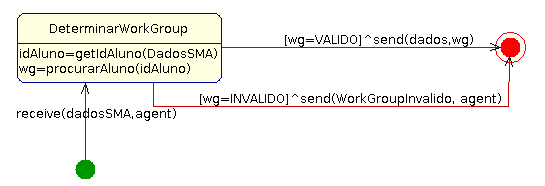
\includegraphics[scale=0.48]{images/td-determinar-wg.png}
	\caption{Detalhamento da tarefa ``Determinar WG do Aluno'' que pertence à regra~\emph{Manager}.}
	\label{fig:td-determinar-wg}
\end{figure}

O diagrama da tarefa ``Criar Workgroup'' da regra~\emph{Manager} apresentado na Figura~\ref{fig:td-criar-wg} inicia com entrada de uma mensagem vinda da tarefa~\emph{studentInterface} e a mudança para o estado ``criarWorkgroup''. O estado cria os agentes cognitivo, metacognitivo, afetivo e o workgroup propriamente dito. Por fim, caso o workgroup seja válido, ou seja, não tenha ocorrido nenhum erro durante a criacão, é enviado um código de sucesso à tarefa~\emph{studentInterface}. Caso contrário, o workgroup deve ser criado novamente.

\begin{figure}
	\centering
	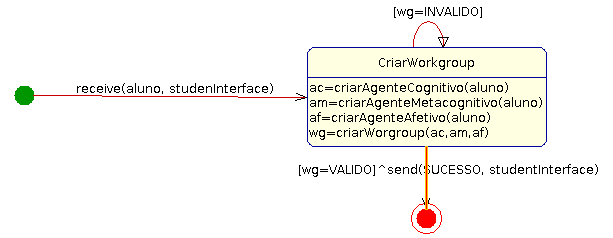
\includegraphics[scale=0.48]{images/td-criar-wg.png}
	\caption{Detalhamento da tarefa ``Criar Workgroup'' que pertence à regra~\emph{Manager}.}
	\label{fig:td-criar-wg}
\end{figure}

Agora na regra~\emph{StudentWorgroup}, o diagrama da tarefa ``Processar Dados'' apresentado na Figura~\ref{fig:td-criar-wg} mostra que o modelos do aluno são separados e enviados junto com os dados do SMA para os respectivos agentes.

\begin{figure}
	\centering
	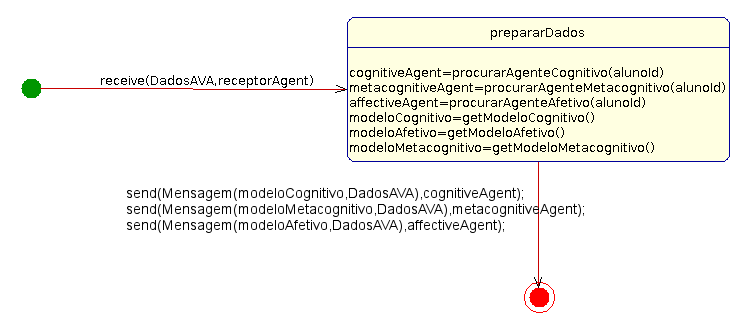
\includegraphics[scale=0.48]{images/td-processar-dados.png}
	\caption{Detalhamento da tarefa ``Processar Dados'' que pertence à regra~\emph{StudentWorkgroup}.}
	\label{fig:td-processar-dados}
\end{figure}

A Figura~\ref{fig:td-atualizar-modelos} apresenta o diagrama da tarefa ``Atualizar Modelos'', representando o recebimento das inferências cognitiva, metacognitiva e afetiva. A transição inicia-se com o recebimento de um desses modelos. A tarefa vai para o estado ``Aguardar Modelo Completo'', onde verifica se os três modelos já foram inferidos. Se a verificação for válida, a tarefa é terminada e o objetivo de inferência dos modelos é atingido. Caso contrário, a tarefa aguarda as outras inferências e muda seu estado quando elas chegarem, repetindo assim o fluxo inicial.

\begin{figure}
	\centering
	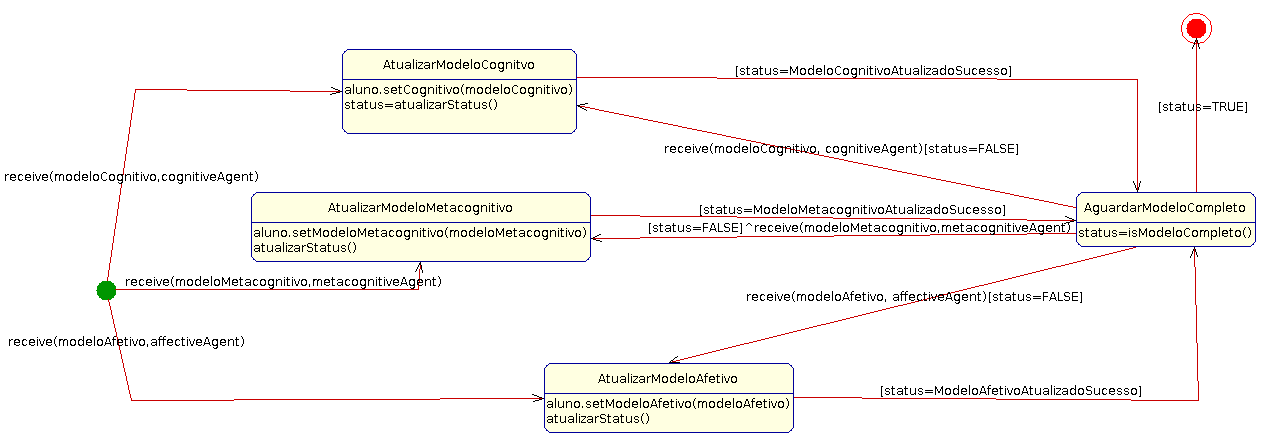
\includegraphics[scale=0.4]{images/td-atualizar-modelos.png}
	\caption{Detalhamento da tarefa ``Atualizar Modelos'' que pertence à regra~\emph{StudentWorkgroup}.}
	\label{fig:td-atualizar-modelos}
\end{figure}

As regras~\emph{AffectiveAction} e~\emph{MetacognitiveAction} possuem tarefas semelhantes. A Figura~\ref{fig:td-inferir-afetivo} mostra o recebimento da mensagem do~\emph{workgroup} e a realização da inferência afetiva. A Figura~\ref{fig:td-inferir-metacognitivo} mostra o comportamento semelhante para a inferência metacognitiva. Devido ao objetivo deste trabalho não ser estudar especificamente essas inferências, mas, criar a arquitetura do SMA Frank, foi previsto apenas os agentes e a etapa de inferência dos modelos.

\begin{figure}
	\centering
	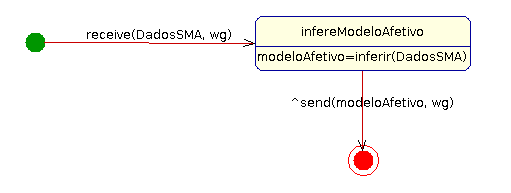
\includegraphics[scale=0.48]{images/td-inferir-afetivo.png}
	\caption{Detalhamento da tarefa ``Inferir Modelo Afetivo'' que pertence à regra~\emph{AffectiveAction}.}
	\label{fig:td-inferir-afetivo}
\end{figure}

\begin{figure}
	\centering
	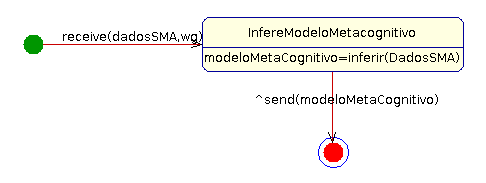
\includegraphics[scale=0.48]{images/td-inferir-metacognitivo.png}
	\caption{Detalhamento da tarefa ``Inferir Modelo Metacognitivo'' que pertence à regra~\emph{MetacognitiveAction}.}
	\label{fig:td-inferir-metacognitivo}
\end{figure}

A regra~\emph{CognitiveAction} possui um detalhamento maior, visto que será necessário a inferência explícita do estilo de aprendizagem do aluno. Para tanto, as regras possuem uma comunicação interna (representada pela linha tracejada azul) significando que provavelmente estarão no mesmo agente. De forma simples as tarefas da regra~\emph{CognitiveAction} ``Separar Dados de Aprendizagem'' e ``Atualizar Modelo'' fazem o semelhante que já foi mostrado em outras tarefas. Portanto, o diagrama destas tarefas foi suprimido.
%%%%Suprimi as tarefas

O diagrama da regra~\emph{LearningMethodAnalyzer} apresentado na Figura~\ref{fig:td-analise-aprendizagem} mostra o processo de análise do estilo de aprendizagem. A inferência deve ser do tipo explícita caso os dados sejam o questionário. Caso contrário, a inferência deve ser implícita e pode variar de acordo com o AVA que enviou os dados.
\begin{figure}
	\centering
	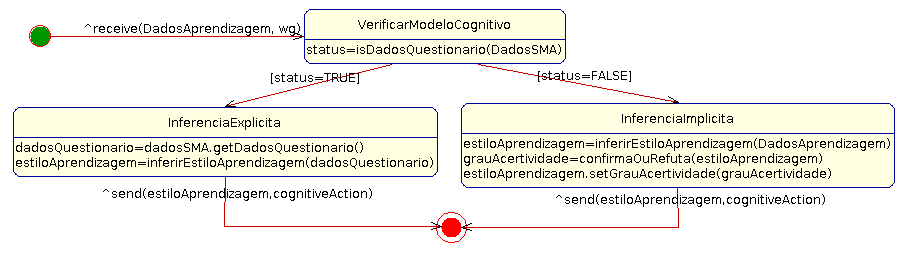
\includegraphics[scale=0.48]{images/td-analise-aprendizagem.png}
	\caption{Detalhamento da tarefa ``Analisar Estilo de Aprendizagem'' que pertence à regra~\emph{LearningMethodAnalyzer}.}
	\label{fig:td-analise-aprendizagem}
\end{figure}

\subsection{Projeto}\label{subsection:design}

Após a conclusão da primeira etapa do MASE, é necessário definir as classes dos agentes, bem como as suas conversações. A Figura~\ref{fig:agent-class-diagram} apresenta o diagrama de classes do SMA. Nele é possível identificar arquitetura a do SMA Frank, composta pelos seguintes agentes:

\begin{figure}
	\centering
	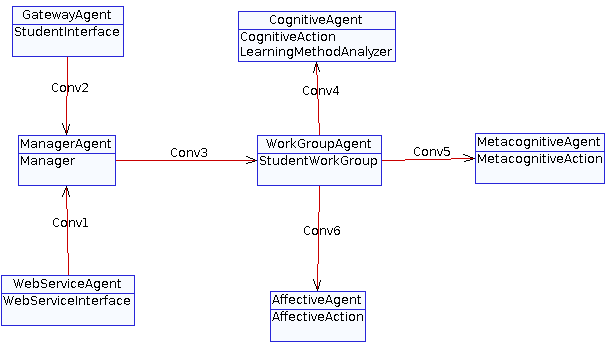
\includegraphics[scale=0.48]{images/agent-class-diagram.png}
	\caption{Diagrama de Classes do SMA Frank.}
	\label{fig:agent-class-diagram}
\end{figure}

\begin{itemize}
	\item GatewayAgent - Possui a regra StudentInterface, responsável pela interface com a plataforma~\emph{web}, ou seja, com o estudante e o docente.
	\item WebServiceAgent - Possui a regra~\emph{WebServiceInterface}, é responsável pela interface com os AVA.
	\item ManagerAgent - Possui a regra~\emph{Manager}, é responsável pela gerência da plataforma: Criação dos agentes, encaminhamento de mensagens.
	\item WorkgroupAgent - Possui a regra~\emph{StudentWorkgroup}, responsável pela gerência do grupo de trabalho de um determinado aluno.
	\item CognitiveAgent - Possui as regras~\emph{CognitiveAction},~\emph{LearningStyleAction}. Responsável pela inferência do modelo cognitivo do aluno.
	\item AffectiveAgent - Possui a regra~\emph{AffectiveAction}. Responsável pela inferência do modelo afetivo do aluno.
	\item MetacognitiveAgent - Possui a regra~\emph{MetacognitiveAction}. Responsável pela inferência do modelo metacognitivo do aluno.
\end{itemize}

As conversações são definidas da seguinte forma:
\begin{itemize}
	\item Conv1 - Conversação do~\emph{WebServiceAgent} com o~\emph{ManagerAgent}
	\item Conv2 e Conv7 - Conversação do~\emph{GatewayAgent} com o~\emph{ManagerAgent}
	\item Conv3 - Conversação do~\emph{ManagerAgent} com o~\emph{WorkgroupAgent}
	\item Conv4, Conv5 e Conv6 - Conversação do~\emph{WorkGroupAgent} com os agentes~\emph{CognitiveAgent},~\emph{MetacognitiveAgent} e~\emph{AffectiveAgent}, respectivamente.
\end{itemize}

A primeira conversação (conv1) ocorre de forma simples. A Figura~\ref{fig:conv1-iniciador} representa a conversação do lado iniciador da conversação. Ele solicita ao respondedor a verificação da existência do aluno na plataforma e entra no estado de espera. Caso a resposta seja~\emph{usuarioValido}, o iniciador irá enviar a mensagem~\emph{enviarDados} e encerrar a execução normalmente. Caso contrário, entrará no estado de falha, onde informará erro de execução.
\begin{figure}
	\centering
	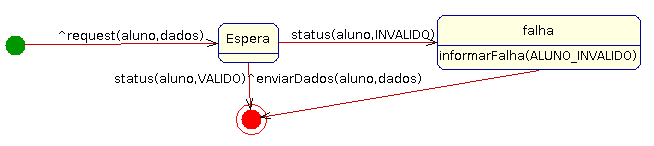
\includegraphics[scale=0.48]{images/conv1-iniciador.png}
	\caption{Detalhamento da Conversação 1 no lado do Iniciador.}
	\label{fig:conv1-iniciador}
\end{figure}
O lado respondedor da conversação, representado na Figura~\ref{fig:conv1-respondedor}, inicia-se com o request do iniciador e o estado ``Verificar'', onde é identificada a existência do aluno. Por fim, é enviado uma resposta sobre a existência do aluno para o iniciador da conversaçào.

\begin{figure}
	\centering
	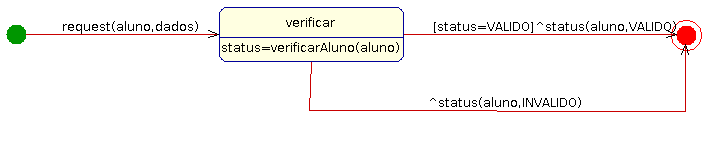
\includegraphics[scale=0.48]{images/conv1-recebedor.png}
	\caption{Detalhamento da Conversação 1 no lado do Respondedor.}
	\label{fig:conv1-respondedor}
\end{figure}

A segunda conversação (conv2) possui a mesma dinâmica da conversação 1, portanto seu diagrama será suprimido.

A conversação 3 (conv3) é bastante simples. Não há nenhum estado de transição durante a conversação, pois é apenas um encaminhamento de dados para o grupo de trabalho do aluno.

As conversações 4, 5 e 6 (conv4, conv5 e conv6) possuem dinâmica bastante semelhante, sendo representado aqui somente a conversação 4 na Figura~\ref{fig:conv4-iniciador}. Do lado iniciador da conversação, ele envia um request com o modelo a ser inferido, os dados a serem analisados e entra em estado de espera. Em seguida, quando receber a resposta, ele atualiza o modelo cognitivo.
\begin{figure}
	\centering
	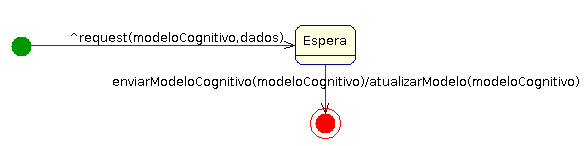
\includegraphics[scale=0.48]{images/conv4-iniciador.png}
	\caption{Detalhamento da Conversação 4 no lado iniciador.}
	\label{fig:conv4-iniciador}
\end{figure}

O lado do recebedor, apresentado na Figura~\ref{fig:conv4-recebedor}, recebe o~\emph{request} e infere o modelo do aluno. Por fim, apenas reenvia novamente ao iniciador da conversação.
\begin{figure}
	\centering
	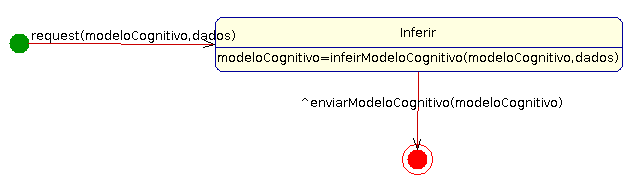
\includegraphics[scale=0.48]{images/conv4-recebedor.png}
	\caption{Detalhamento da Conversação 4 no lado iniciador.}
	\label{fig:conv4-recebedor}
\end{figure}

A Figura~\ref{fig:conv7-iniciador} apresenta a última conversação, conv7, consiste da conversação necessária para criação do grupo de trabalho do aluno. No lado do iniciador, ele requisita a verificação da existência do aluno no ambiente. Caso não exista, ele envia a resposta de criação do grupo de trabalho para o recebedor da conversação.
\begin{figure}
	\centering
	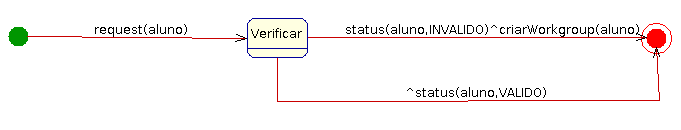
\includegraphics[scale=0.48]{images/conv7-iniciador.png}
	\caption{Detalhamento da Conversação 7 no lado iniciador.}
	\label{fig:conv7-iniciador}
\end{figure}

O lado recebedor, representado na Figura~\ref{fig:conv7-recebedor}, é iniciado com o~\emph{request} e faz a verificação da existência do aluno. Caso já exista, a conversação é encerrada. Caso contrário, ele entra no estado de espera e em seguida faz a criação do workgroup.
\begin{figure}
	\centering
	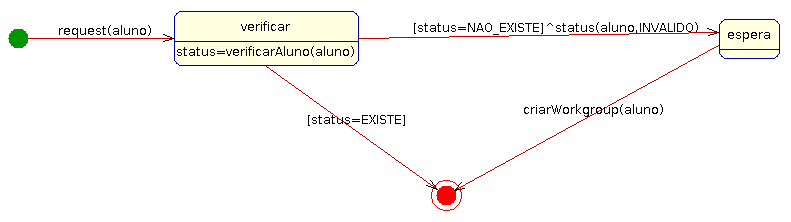
\includegraphics[scale=0.48]{images/conv7-recebedor.png}
	\caption{Detalhamento da Conversação 7 no lado recebedor.}
	\label{fig:conv7-recebedor}
\end{figure}

A arquitetura de deploy do trabaho deve ser dinâmica, visto que os agentes de trabalho devem ser instânciados dinâmicamente. Funcionando em ambiente descentralizado, o SMA Frank precisa balancear a carga de uso entre os ambientes disponíveis. Dessa forma, o diagrama de deploy foi desnecessário.

\section{Arquitetura}\label{section:arquitetura}

A arquitetura do sistema foi separada em duas aplicações: A parte~\emph{web} chamada de~\emph{Frank Web} e a parte multiagente chamada de~\emph{SMA Frank}. Esta seção pretende relatar a arquitetura interna de cada parte, bem como as dificuldades encontradas na integração entre ambas.

A solução foi separada devido aos seguintes aspectos:
\begin{itemize}
	\item Maior Distribuição - É possível replicar a parte~\emph{web} em vários nós de uma rede, possibilitando assim um maior ganho de performance da aplicação.
	\item Menor Complexidade - Os objetivos das aplicações estão separados, modularizando assim as responsabilidades de cada parte.
	\item Menor Dificuldade - A parte~\emph{web} é responśavel pela interação com o usuário e com o banco de dados. Estes pontos seriam muito mais difíceis de implementar no framework JADE.
\end{itemize}

A Figura~\ref{fig:arquitetura-frank} apresenta a arquitetura geral da solução, onde é possível identificar as duas aplicações distintas: Frank Web e Frank SMA. A aplicação~\emph{web} faz a interface com o estudante e o docente. A plataforma~\emph{web} comunica-se com o SMA através do agente~\emph{GatewayAgent}, que reencaminha as informações para o agente~\emph{Manager}, responsável pela gerência da plataforma. Em um mesmo ambiente do Frank, é possível existir inúmeros agentes~\emph{managers}. Este agente consegue comunicar-se com todos os grupos de trabalho registrados que podem, ou não, estar na mesmo~\emph{container} que ele. São permitidos inúmeros~\emph{containers} que não necessariamente estarão na mesma máquina do~\emph{container} principal. O grupos de trabalho é criado individualmente por aluno, sendo composto pelos agentes ``AA'' (Agente Afetivo), ``AC'' (Agente Cognitivo), ``AM'' (Agente Metacognitivo) e o próprio ``GT'' (Grupo de trabalho).
\begin{figure}
	\centering
	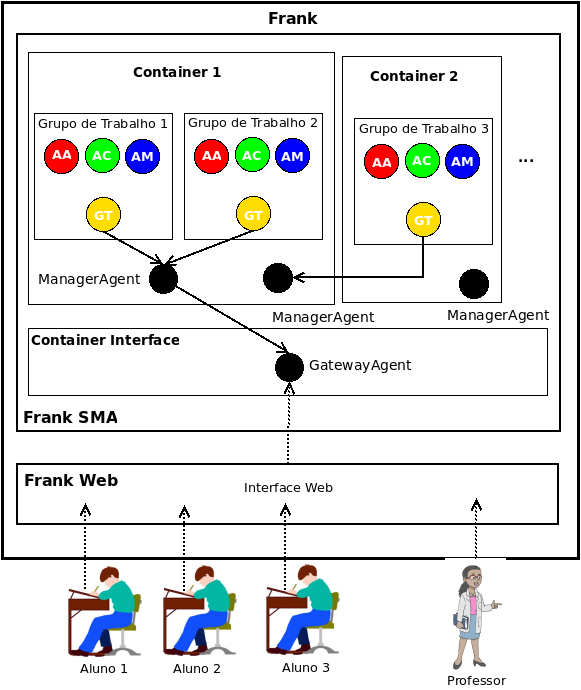
\includegraphics[scale=0.6]{images/arquitetura-frank.png}
	\caption{Representação da arquitetura da solução.}
	\label{fig:arquitetura-frank}
\end{figure}

\subsection{Frank Web}
A parte~\emph{web} utiliza-se do framework JBoss Seam, confome dito anteriormente, um framework que acelera o tempo de desenvolvimento de aplicações dinâmicas para a~\emph{web}. Para facilitar a manutenção do código e a reescrita de alguma parte dele, foi adotado o padrão de projetos
Model View Controller (MVC). Esse padrão divide a arquitetura do sistema em três partes:

\begin{itemize}
	\item Apresentação - Responsável pela apresentação dos dados para o usuário em uma página~\emph{web}.
	\item Controladora - Determina o componente a ser executado.
	\item Modelo - Representação das entidades, auxiliam na interação com o banco dados.
\end{itemize}

As ferramentas disponibilizadas pelo framework geraram todo o código para visualização, inserção, atualização e exclusão de dados. Além disso, geraram todas as páginas para que o usuário possa interagir com o sistema. 

Após a geração do código inicial, foi necessário implementar algumas funcionalidades específicas da aplicação Frank-Web. A primeira delas foi implementar a ação de autenticação conjunta com o SMA. Quando o aluno fizer login no sistema, a aplicação~\emph{web} envia uma mensagem ao SMA para a criação do grupo de trabalho.

Em seguida, foi necessário a implementação a tela de respostas do questionário feita pelo usuário.

Por fim, a implementação da tela de notificação ao docente do estilo de aprendizagem do aluno.

\subsection{SMA Frank}

O SMA Frank foi desenvolvido com o~\emph{middleware} JADE, devido a grande aceitação na comunidade de sistemas e o extenso suporte. A aplicação está divida entre os agentes criados e os seus comportamentos (justificados na seção anterior).

A comunicação entre os agentes foi implementada por meio de ontologias de comunicação da plataforma JADE. O pacote de ontologia do~\emph{framework} permite a criação de abstrações muito robustas, descartando neste primeiro momento a utilização de bibliotecas de terceiros.

No JADE, os agentes devem adicionar comportamentos, que são disparados quando o agente recebe uma mensagem. Os comportamentos são separados conforme o objetivo do agente.

Foram implementadas duas ontologias. A primeira, chamada de~\emph{FrankManagementOntology}, tem a função de gerenciamento da plataforma. Logo as ações de criação e destruição de agentes estarão presentes nela.

A ontologia~\emph{ModelInferOntology} possui a função de modelar todos os conceitos relacionados à inferência do modelo do aluno. Portanto, conceitos como estilo de aprendizagem, modelo cognitivo, afetivo e metacognitivo devem estar nesta ontologia. É importante ressaltar que os modelos não estão completos, sendo necessário que em trabalhos futuros sejam definidas as ontologias.

\subsection{Aspectos da Integração}

A integração entre o~\emph{Frank Web} e o~\emph{SMA Frank} pareceu bastante complexa em uma análise inicial. Por não compartilhar a mesma Máquina Virtual Java ou~\emph{Java Virtual Machine} (JVM), a dificuldade de integração pareceu alta.

O Jade porém possui uma forma nativa em que aplicações externas podem se conectar com o ambiente em execução. A classe~\emph{DynamicJadeGateway} registra um agente na plataforma, que atuará como uma ponte entre a aplicação e o ambiente de execução.

Esse agente funcionará de forma distinta dos outros agentes da plataforma. O agente não receberá mensagens da aplicação~\emph{web}, ao invés disso receberá objetos JAVA que representarão comandos. Para os diferentes comandos, o agente pode lançar diferentes mensagens na plataforma SMA. A aplicação~\emph{Frank SMA} implementa 6 comandos:

\begin{itemize}
	\item AnswerCommand
	\item CreateAgentCommand
	\item DestroyAgentCommand
	\item DimensionCommand
	\item ProcessQuestionnaireCommand
	\item RequestCognitiveModelCommand
\end{itemize}

Neste capítulo foram apresentados todos os aspectos da modelagem da solução: as duas fases da metodologia com todos os diagramas inerentes. Além disso, a arquitetura solução foi definida de forma a dividir o sistema em duas aplicações distintas. O próximo capítulo contém a apresentação do protótipo da solução proposta, bem como os resultados obtidos.























